% Define the document type and font size
\documentclass[12pt]{article}

\usepackage[spanish]{babel} % Package for the Spanish language
\usepackage[utf8]{inputenc} % Package for UTF-8 character encoding
\usepackage{geometry} % Package to configure document margins
\usepackage{listings} % Package to include source code in the document
\usepackage{xcolor} % Package to define colors
\usepackage{fancyhdr} % Package to customize headers and footers
\usepackage{amsmath} % Package for advanced mathematical symbols and environments
\usepackage{amssymb} % Package for additional mathematical symbols
\usepackage{graphicx} % Package to include graphics
\usepackage{multirow} % Package to create tables with multiple rows
\usepackage{ragged2e} % Package to justify text
\usepackage{pdflscape} % Package to create landscape pages

\setlength{\parskip}{1em} % Space between paragraphs
\setlength{\parindent}{0pt} % Without indentation for paragraphs

% Definition of colors for source code
\definecolor{KEYWORDS}{HTML}{0000ff}
\definecolor{COMMENTS}{HTML}{888888}
\definecolor{STRINGS}{HTML}{ff0000}

% Configuration of the listings environment to display source code
\lstset{
	frame=shadowbox,
	language=c++,
	aboveskip=3mm,
	belowskip=3mm,
	xleftmargin=10mm,
	xrightmargin=10mm,
	showstringspaces=false,
	columns=flexible,
	basicstyle={\small\ttfamily},
	numbers=left,
	numberstyle=\tiny\color{COMMENTS},
	keywordstyle=\color{KEYWORDS},
	commentstyle=\color{COMMENTS},
	stringstyle=\color{STRINGS},
	breaklines=true,
	breakatwhitespace=true,
	tabsize=4
}

% Configuration of document margins
\geometry{
	a4paper,
	left=25mm,
	right=25mm,
	top=25mm,
	bottom=25mm
}

\title{Proyecto Cacerola - Modelado del Dominio} % Document title
\author{Druxorey} % Document author
\date{\today} % Document date

\begin{document}

\begin{titlepage}
	\centering
	\vspace{1cm}
	{\large {Universidad Central de Venezuela}\par}
	{\large {Facultad de Ciencias}\par}
	{\large {Escuela de Computación}\par}
	{\large {Ingeniería de Software}\par}
	\vspace{6cm}
	{\LARGE \textbf{Disciplina de Requisitos}\par}
	\vspace{0.25cm}
	{\Large \textbf{Entrega 2}\par}
	\vfill
	\begin{flushleft}
		{\large Profesor: Marcel Castro\par\vspace{-0.5em}}
		{\large Sección: C2\par\vspace{-0.5em}}
		{\large Equipo \#2\par\vspace{-1em}}
		\begin{itemize}
			\item Guillermo Galavís\vspace{-0.5em}
			\item José Apure\vspace{-0.5em}
			\item Renzo Morales\vspace{-0.5em}
			\item Luis David Lima\vspace{-0.5em}
		\end{itemize}
	\end{flushleft}
	\vspace{0.5cm}
	\centering
	{\large \today\par}
\end{titlepage}

\section{Visión del Producto}

\vspace{1cm}
\begin{table}[htbp]
\centering
\begin{tabular}{|p{3.5cm}|p{3.5cm}|p{3.5cm}|p{3.5cm}|}
\hline
\textbf{Nombre Clave}			  & \multicolumn{3}{p{8cm}|}{\textbf{Frase Representativa}}												  \\ \hline
\multicolumn{1}{|p{3.5cm}|}{MiComedorUCV} & \multicolumn{3}{p{8cm}|}{Sistema para la gestión eficiente del comedor universitario}					\\ \cline{1-4}
\textbf{Grupo de Usuarios}		 & \multicolumn{1}{p{3.5cm}|}{\textbf{Necesidades}} & \multicolumn{1}{p{3.5cm}|}{\textbf{Producto}} & \textbf{Valor} \\ \cline{1-4}
\begin{tabular}[c]{@{}p{3.5cm}@{}}- Estudiantes pertenecientes a la Universidad Central de Venezuela.\\ - Personal Docente.\\ - Personal Administrativo.\\ - Personal Obrero.\end{tabular} &
\begin{tabular}[c]{@{}p{3.5cm}@{}}- Consultar el menú semanal disponible.\\ - Acceder al comedor en turnos asignados.\\ - Conocer los horarios de los turnos de comida.\\ - Obtener reportes del consumo y demanda.\\ - Gestionar los insumos y menús semanalmente.\\ - Evitar largas filas al ingresar al comedor.\\ - Saber si el usuario tiene un cupo en un turno específico.\end{tabular} &
\begin{tabular}[c]{@{}p{3.5cm}@{}}- Permitir consultar el menú semanal.\\ - Gestionar la asignación de turnos y cupos.\\ - Visualizar la información de turnos de comida.\\ - Generar reportes de consumo y demanda.\\ - Administrar los insumos y la planificación de menús.\\ - Validar la reserva de cupos por usuario.\\ - Registrar nuevos usuarios (estudiantes, docentes, administrativos, obreros).\\ - Controlar el acceso a los turnos programados.\end{tabular} &
\begin{tabular}[c]{@{}p{3.5cm}@{}}- Acceso ágil y sin demoras al comedor.\\ - Mayor control y planificación de sus comidas.\\ - Experiencia de servicio mejorada y más cómoda.\\ - Optimización de la gestión de recursos e insumos.\\ - Mejor control del inventario y desperdicio de alimentos.\\ - Mejora en la eficiencia operativa del comedor.\end{tabular} \\ \hline
\end{tabular}
\end{table}

\pagebreak

\section{Diagrama de Casos de Uso}
\vspace{1cm}
\begin{center}
	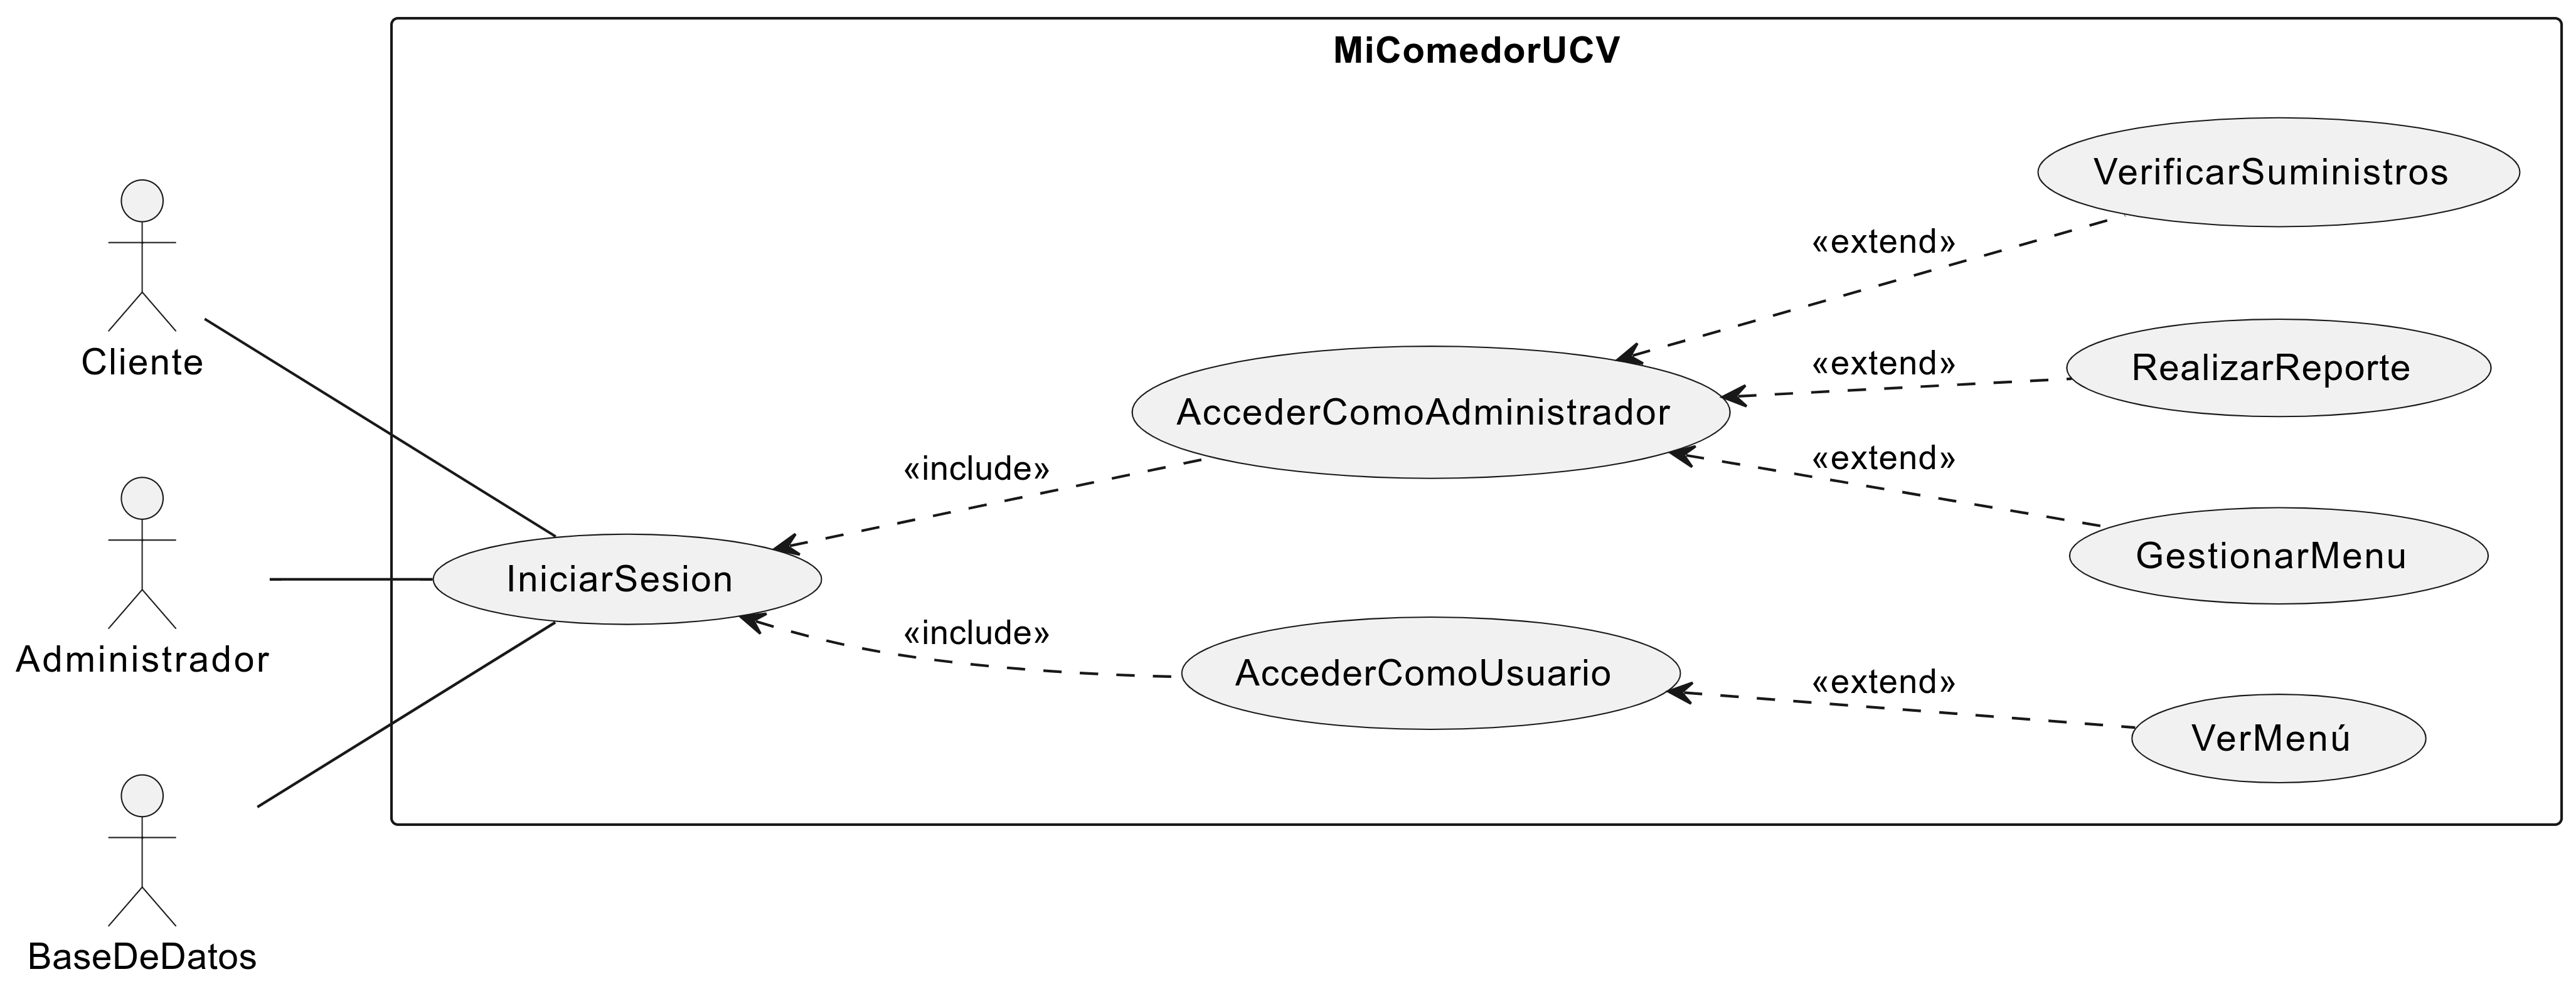
\includegraphics[width=12cm]{Requirements Discipline - Uses Cases Diagram.png}
\end{center}

\pagebreak

\section{Lista de Casos de Uso Prioritario}

\subsection*{Lista de Casos de Uso}

\begin{itemize}
	\item \textbf{Iniciar Sesión}: Este caso de uso permite a los usuarios (\textbf{usuarios} y \textbf{administradores}) acceder al sistema. Es el punto de entrada principal que autentica al usuario y le concede acceso a las funcionalidades correspondientes a su rol. Es un proceso fundamental para la seguridad y la usabilidad del sistema.

	\item \textbf{Registrarse}: Permite a los nuevos \textbf{usuarios} crear una cuenta en el sistema. Se considera una extensión de «Iniciar Sesión» porque un registro exitoso suele llevar al inicio de sesión automático o a la necesidad de iniciar sesión.

	\item \textbf{Ver Turnos}: La funcionalidad central para los \textbf{usuarios}, que les permite a los \textbf{usuarios} conocer los horarios y la disponibilidad de los turnos para el comedor. Esto es esencial para que los usuarios puedan planificar su visita y asegurar su lugar, especialmente en un comedor que maneja horarios específicos o capacidad limitada.

	\item \textbf{Ver Menú}: Permite consultar los platos, bebidas y otras ofertas disponibles en el comedor. Este caso de uso es la razón principal por la que un usuario usaría la aplicación, proporcionando la información necesaria para decidir qué consumir. Es un caso de uso que se incluye dentro de «Ver Turnos».

	\item \textbf{Gestionar Menú}: Este caso de uso es exclusivo para el \textbf{administrador} y le permite realizar todas las operaciones relacionadas con el menú del comedor: añadir nuevos platos, modificar los existentes (precio, descripción, disponibilidad) o eliminarlos. Es vital para mantener la información del menú actualizada y reflejar la oferta real del comedor.

	\item \textbf{Gestionar Turnos}: También exclusivo del \textbf{administrador}, esta funcionalidad le permite crear, modificar o eliminar los turnos disponibles en el comedor. Esto incluye establecer la duración de los turnos, la capacidad de cada uno, y cualquier otra regla asociada, lo cual es crucial para la organización y eficiencia del servicio.

	\item \textbf{Realizar Reporte}: Un caso de uso para el \textbf{administrador} que le permite generar informes sobre diversos aspectos del comedor, como el uso del servicio, la afluencia de usuarios en ciertos turnos, la popularidad de los platos, etc. Estos reportes son herramientas clave para la toma de decisiones, la optimización de recursos y la mejora continua del servicio.

	\item \textbf{Verificar Suministros}: Este caso de uso también es para el \textbf{administrador} y le permite llevar un control y gestión de los inventarios de ingredientes y suministros necesarios para la operación del comedor.
\end{itemize}

\pagebreak

\subsection*{Explicación de los Usuarios}

\begin{itemize}
	\item \textbf{Usuario}: Este es el usuario final del comedor. Su interacción principal con el sistema se centra en la consulta de información y la preparación para hacer uso del servicio. El \textbf{usuario} puede \textbf{ver el turno} (lo que implica también \textbf{ver los menús}) y tiene la capacidad de \textbf{registrarse} e \textbf{iniciar sesión} para acceder a estas funcionalidades. Su rol es fundamental para la operación del comedor, ya que son los beneficiarios directos del servicio.

	\item \textbf{Administrador}: Este usuario tiene un rol de gestión y control sobre el sistema y la operación del comedor. El \textbf{administrador} es el encargado de mantener la información actualizada y de supervisar el funcionamiento del servicio. Sus responsabilidades incluyen \textbf{iniciar sesión}, \textbf{gestionar el menú} (actualizar los platos), \textbf{gestionar los turnos} (establecer la disponibilidad y capacidad), \textbf{realizar reportes} (para análisis y toma de decisiones), y \textbf{verificar los suministros} (para el control de inventario). El administrador asegura que el sistema y el comedor funcionen de manera eficiente.

	\item \textbf{Base De Datos de la UCV}: Aunque no es un usuario humano, este actor representa el \textbf{sistema de información centralizado de la Universidad Central de Venezuela}. Esta base de datos contiene los registros de todos los \textbf{estudiantes, personal docente, administrativo y obrero} que forman parte de la institución.
\end{itemize}

\pagebreak

\section{Especificación de Casos de Uso Prioritarios}
\vspace{1cm}
\begin{center}
\end{center}

\pagebreak

\begin{landscape}
	\section{Diagrama de Contexto}
	\vspace{1cm}
	\begin{center}
		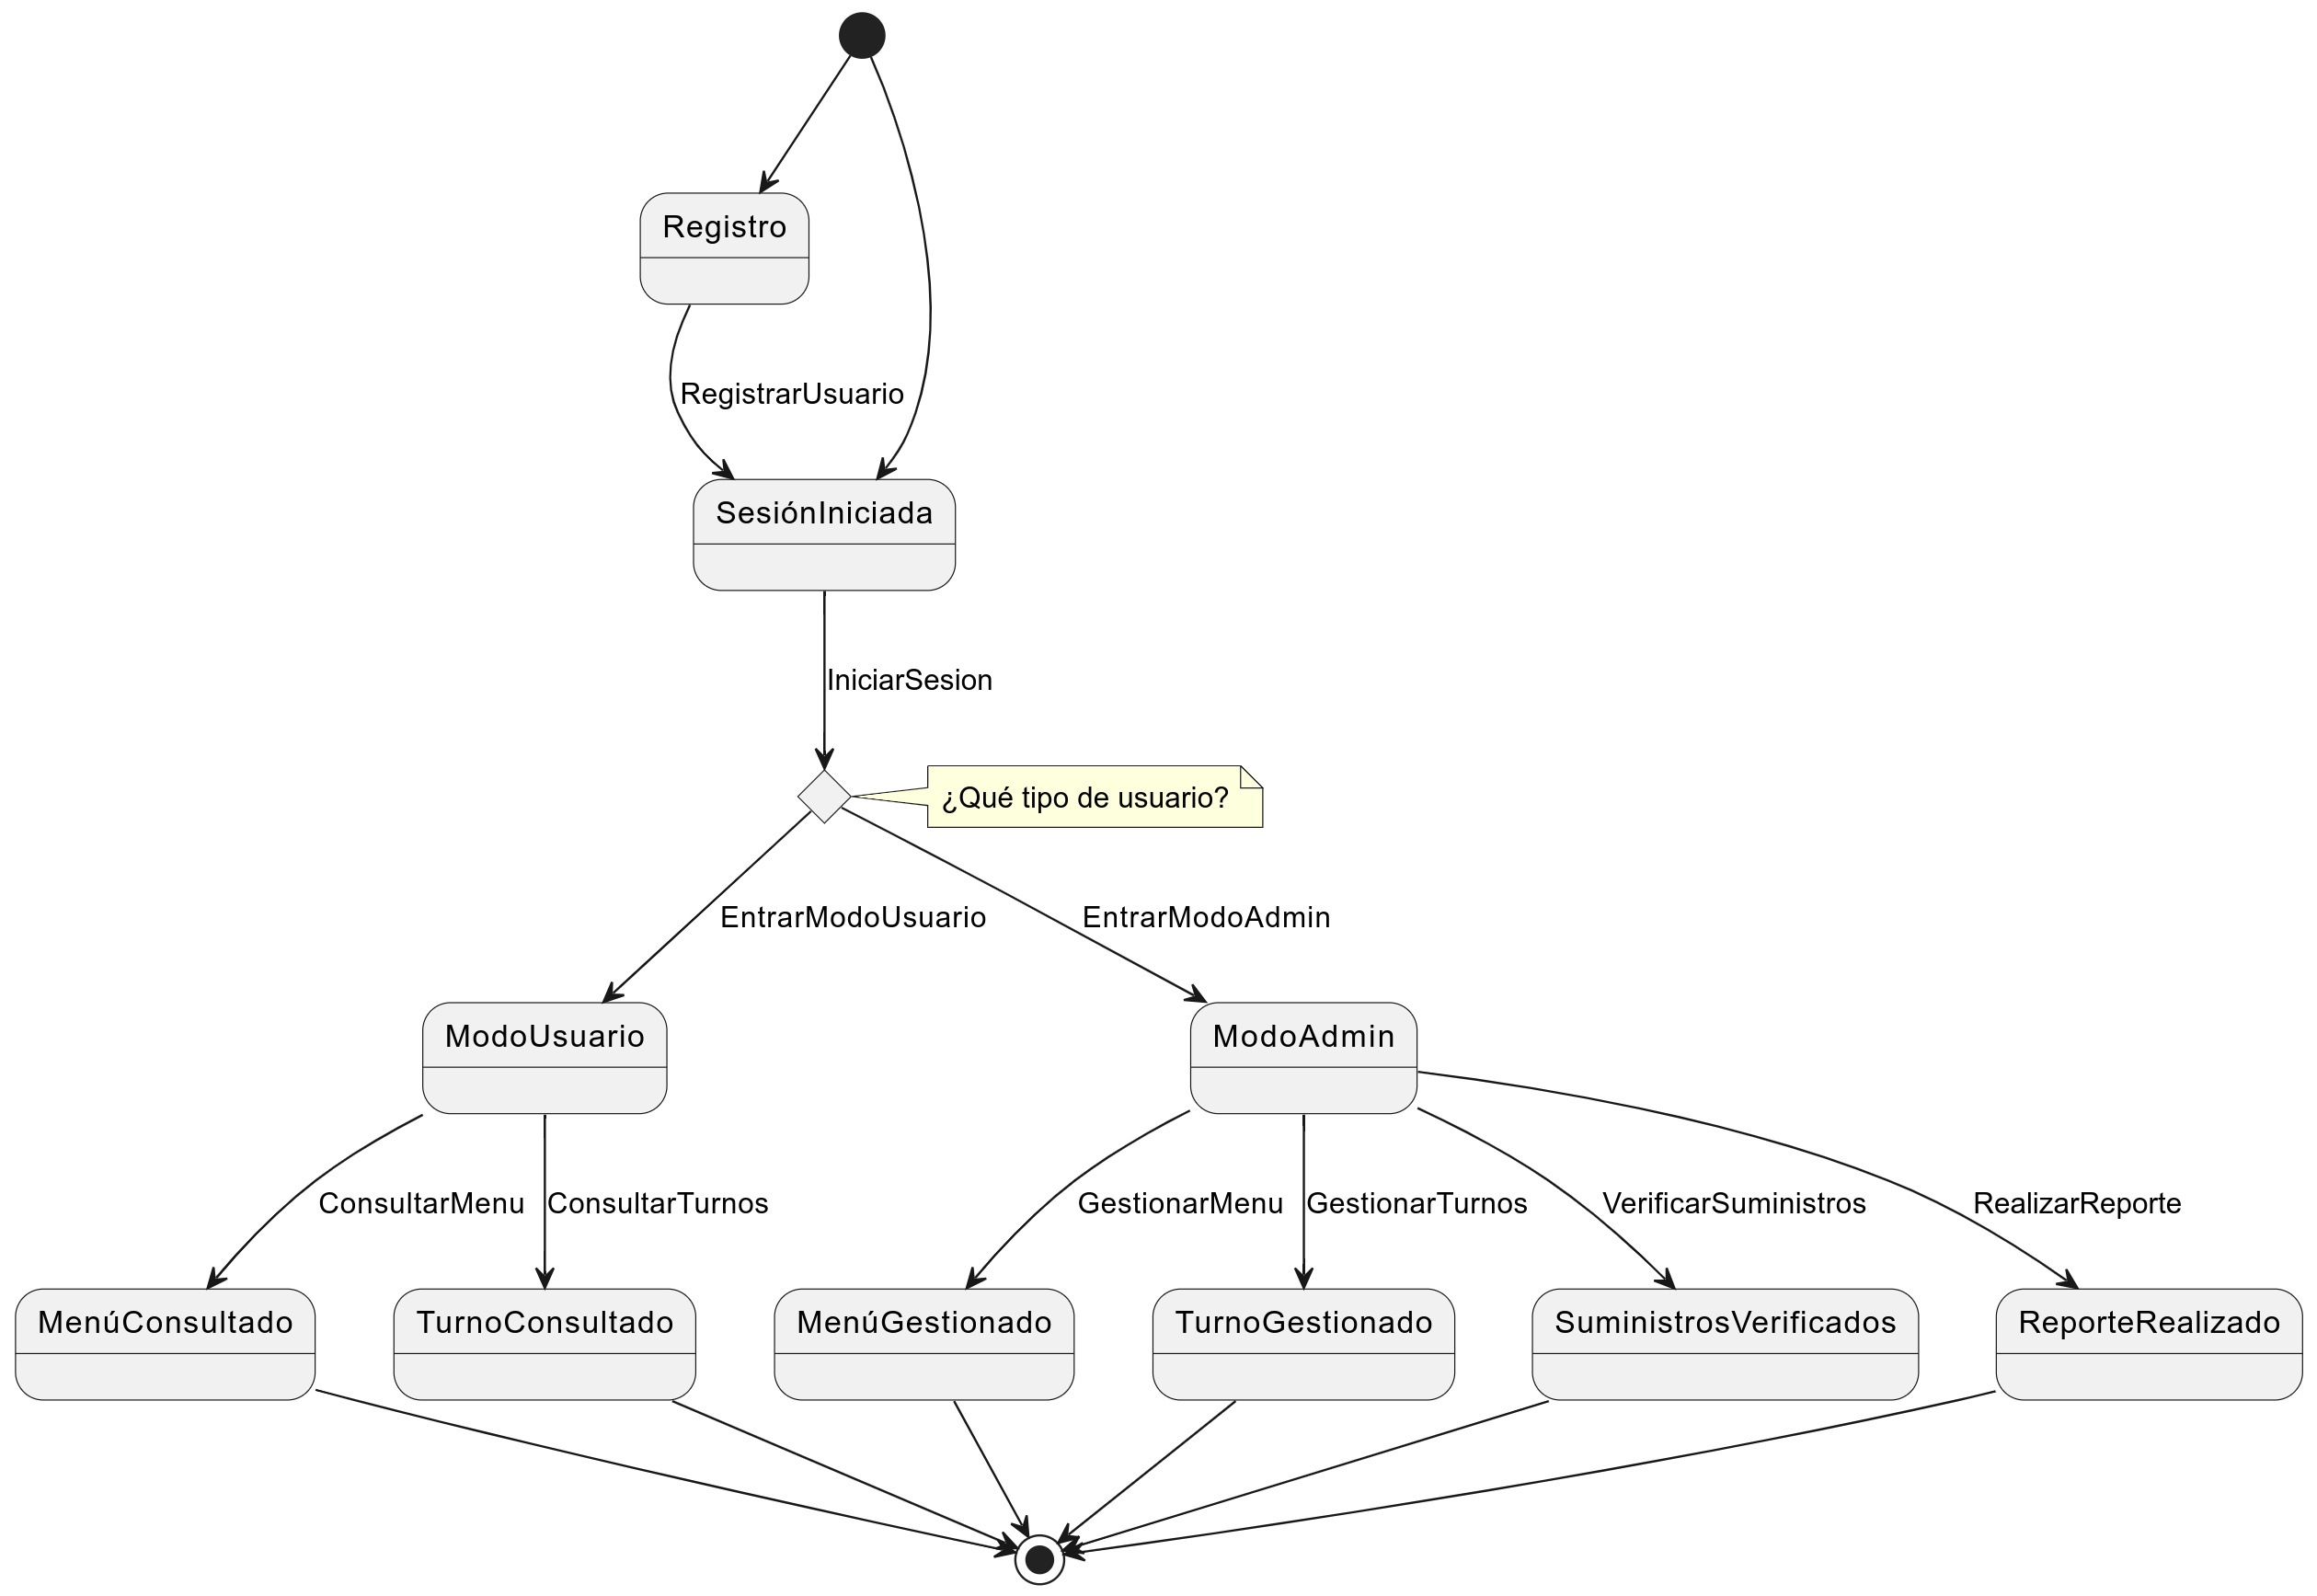
\includegraphics[width=19cm]{Requirements Discipline - Context Diagram.png}
	\end{center}
\end{landscape}

\pagebreak

\section{Prototipo de Interfaz}
\vspace{1cm}
\begin{center}
	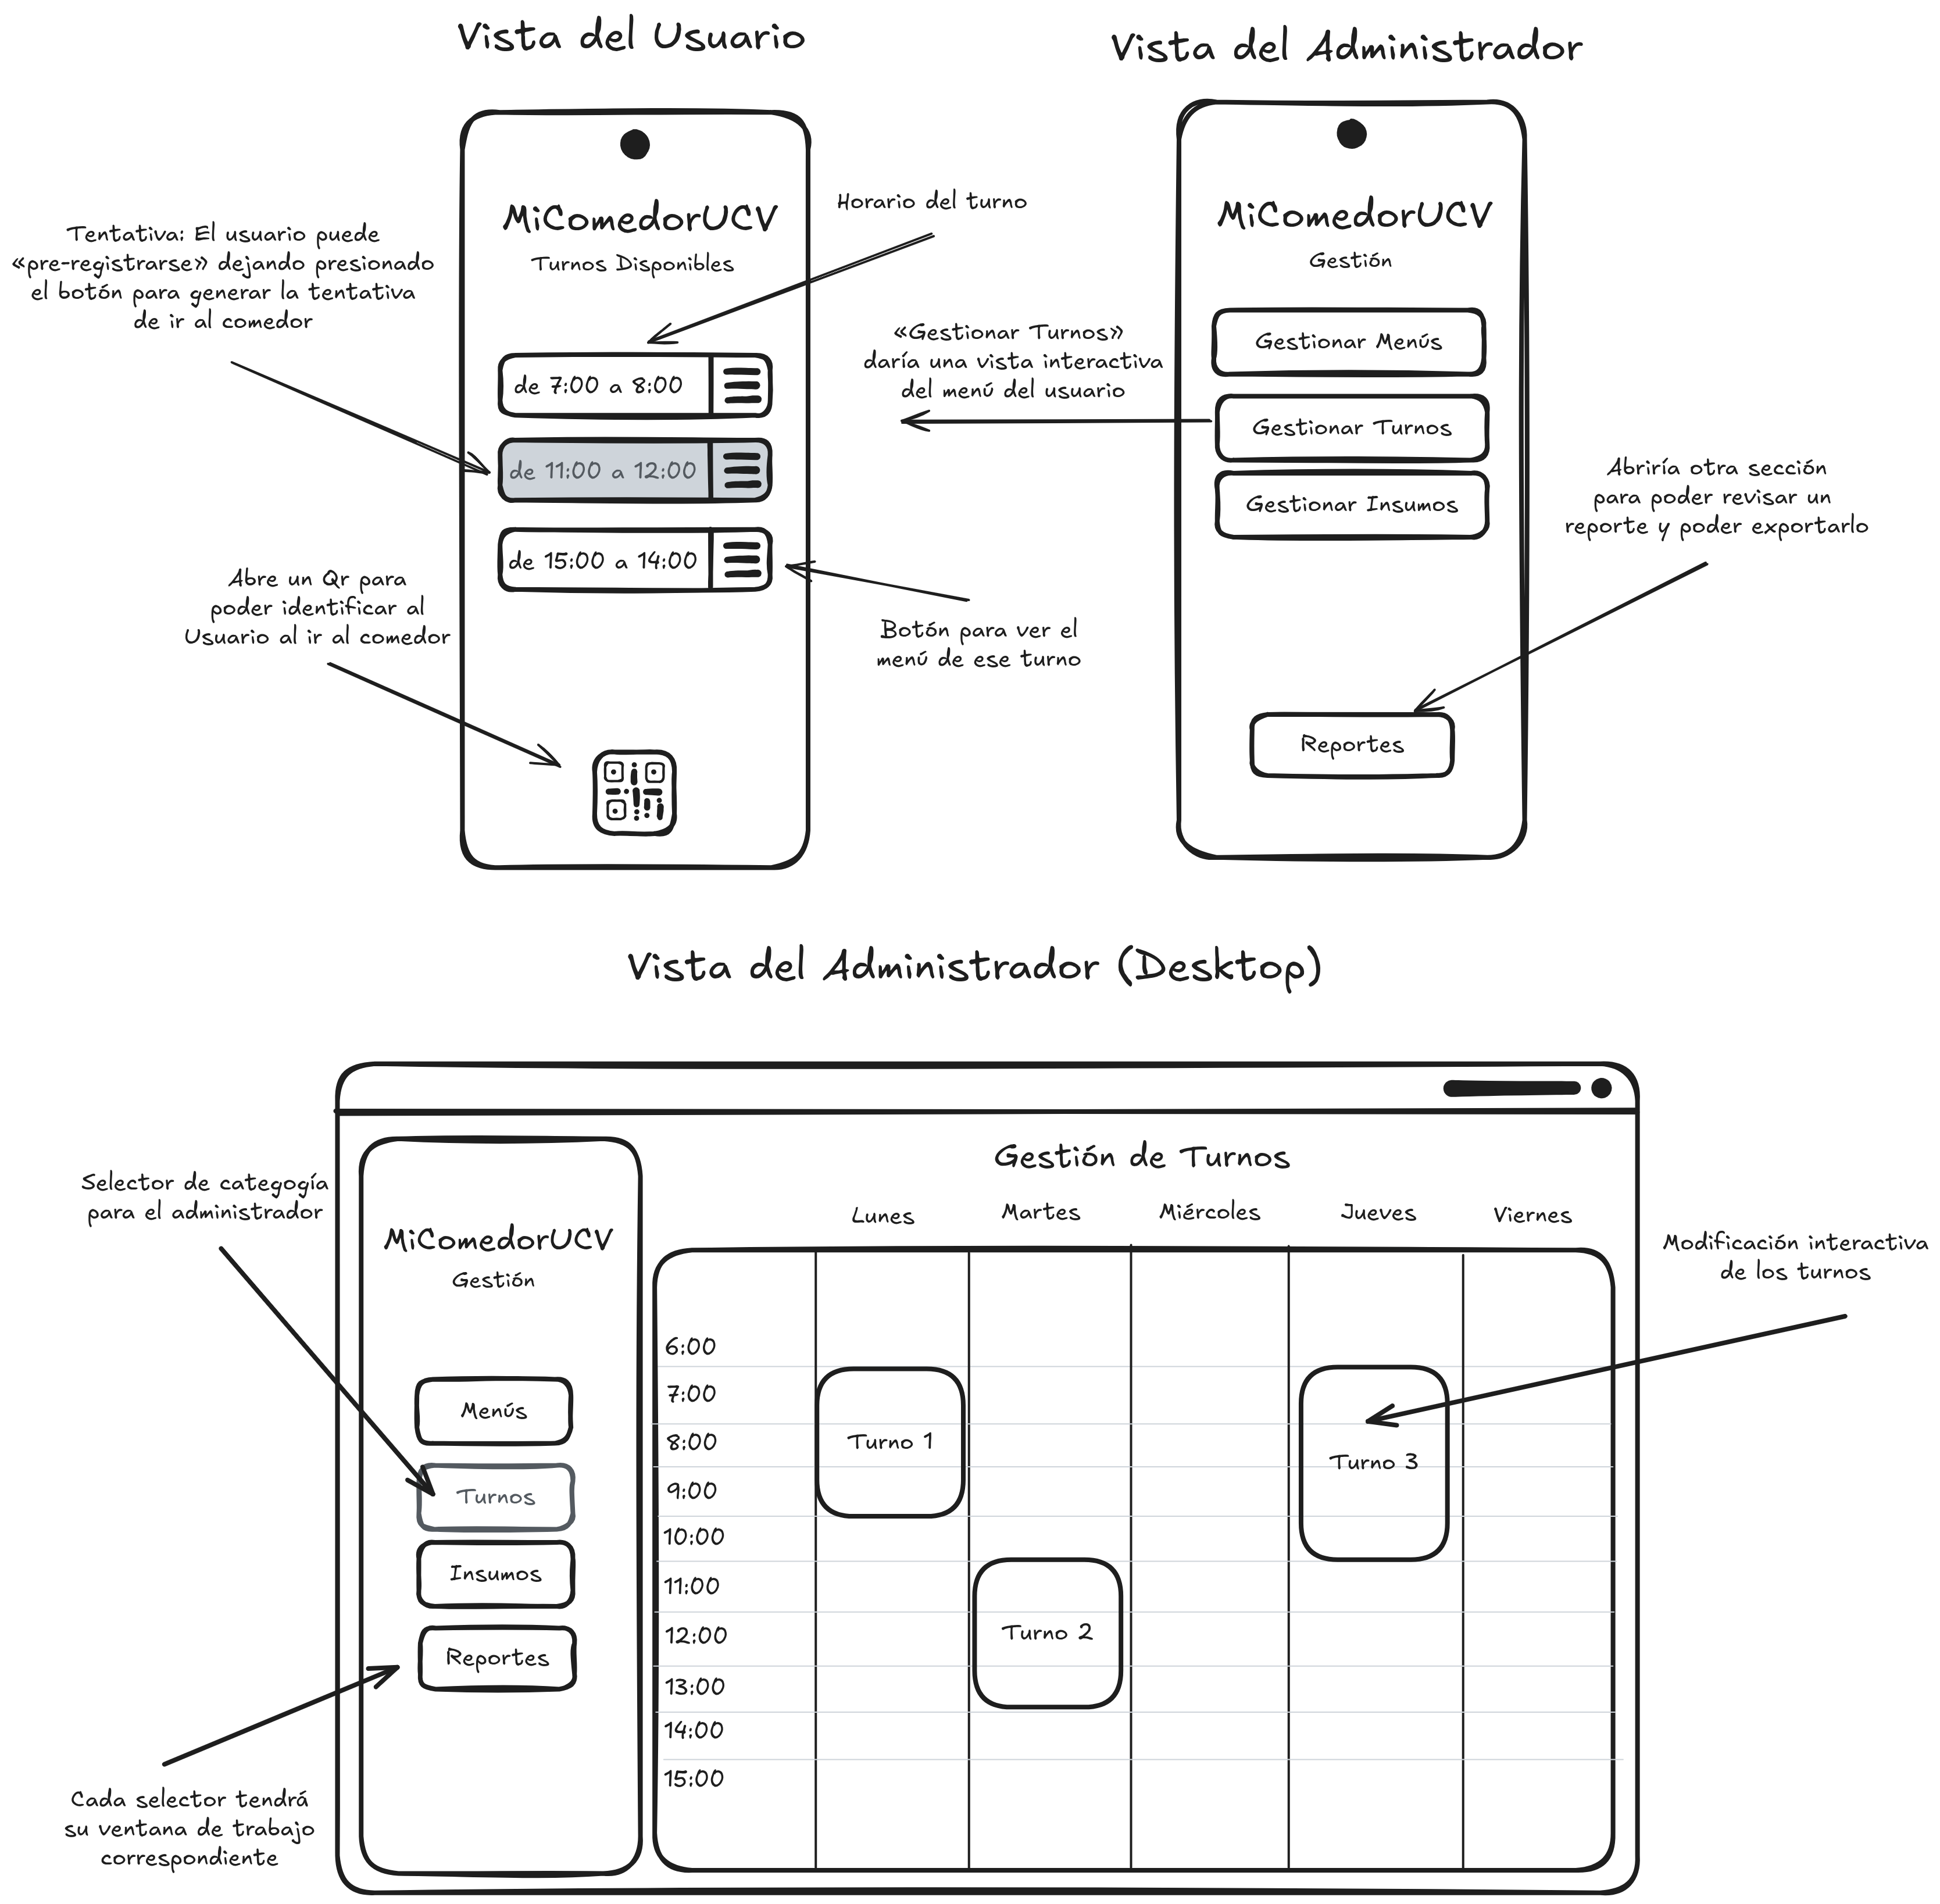
\includegraphics[width=17cm]{Requitements Discipline - Prototipe Wireframe.png}
\end{center}

\end{document}
